\documentclass[12pt]{article}
\usepackage[utf8]{inputenc}
\usepackage{polski}
\usepackage{indentfirst}
\usepackage{graphicx}
\usepackage[]{algorithm2e}
\usepackage{enumerate}

\makeatletter
\renewcommand{\@algocf@capt@plain}{above}
\makeatother

\title{Obliczenia Naukowe \\ \large Lista nr 5}
\author{Eryk Krupa \\ 244993}
\date{}

\begin{document}
\renewcommand{\familydefault}{\sfdefault}
\maketitle
\newpage


\section{Problem}
Rozwiązanie układu równań liniowych: $$Ax = b$$
dla danej macierzy $A \in R^{n\times n}$ 
i wektora prawych stron $b \in R^n$, gdzie $n \geq 4$. \\

Macierz $A$ jest rzadką macierzą blokową o następującej strukturze:

\begin{equation}
A = 
\left(\begin{array}{ccccccc}
A_1 & C_1 & 0 & 0 & 0 & \cdots & 0 \\
B_2 & A_2 & C_2 & 0 & 0  & \cdots & 0 \\
0  & B_3 & A_3 & C_3 & 0  & \cdots & 0 \\
\vdots & \ddots & \ddots & \ddots & \ddots & \ddots & \vdots\\
0   & \cdots & 0  & B_{v-2} & A_{v-2} & C_{v-2} & 0 \\
0  & \cdots & 0  &  0 &B_{v-1} & A_{v-1} & C_{v-1}  \\
0  & \cdots & 0 & 0 & 0& B_{v} & A_{v}  \\ 
\end{array}\right),
\end{equation} 
$v = \frac{n}{l}$, zakładając że $n$ jest podzielne przez $l$, gdzie $l \geq 2$ jest rozmiarem wszystkich kwadratowych macierzy wewnętrznych (bloków) $A_i$, $B_i$, $C_i$, $0$. 



Macierze $A_i$, $B_i$, $C_i$, $0$ są następującej postaci:
\begin{enumerate}[(a)]
\item $A_i \in \R^{l\times l}$,   $i = 1, \ldots,v$ -- macierze gęste,
\item $0 \in \R^{l\times l}$ -- macierz zerowa, 
\item $B_i \in \R^{l\times l}$,   $i = 2, \ldots,v$ -- macierze z niezerowymi dwoma ostatnimi kolumnami:
\begin{equation}
B_i =
\left(\begin{array}{ccccc}
0 & \cdots & 0 & b_{1\,l-1}^i & b_{1\,l}^i \\
0 & \cdots & 0 & b_{2\,l-1}^i & b_{2\,l}^i \\
\vdots & & \vdots & \vdots & \vdots \\
0 & \cdots & 0 & b_{l\,l-1}^i & b_{l\,l}^i \\
\end{array}\right),
\end{equation} 
\item $C_i \in \R^{l\times l}$,   $i = 1, \ldots,v\!-\!1$ -- macierze diagonalne:
\begin{equation}
C_i =
\left(\begin{array}{ccccc}
 c_{1}^i & 0 & 0 & \cdots & 0  \\
0 &  c_{2}^i &  0 & \cdots & 0  \\
\vdots &  \ddots &  \ddots & \ddots & \vdots  \\
0 & \cdots & 0 &  c_{l-1}^i & 0 \\
0 & \cdots & 0 &  0 & c_{l}^i \\
\end{array}\right).
\end{equation} 
\end{enumerate}

Układ $Ax = b$ należało rozwiązać stosując dwie różne metody:
\begin{enumerate}[(a)]
\item metodę eliminacji Gaussa bez wyboru elementu głównego oraz z częściowym wyborem elementu głównego,   
\item metodę eliminacji Gaussa z częściowym wyborem elementu głównego, 
\end{enumerate}

\section{Macierz}
Macierz $A$ dana w zadaniu posiada tylko $(l + 3)n - 3 l$ elementów nie będących zerami. Jest to suma elementów w blokach $A_i$: $v \cdot l^2$, $B_i$: $(v-1) \cdot 2l$ oraz $C_i$: $(v-1) \cdot l$. Oznacza to, że $A$ jest macierzą rzadką. By nie marnować pamięci przechowując macierz w tablicy dwuwymiarowej $n\times n$, użyta została specjalna struktura do przechowywania macierzy rzadkich \texttt{SparseMatrixCSC}, w której macierze przechowywane są w skompresowanym porządku kolumnowym.

\section{Metoda Eliminacji Gaussa}

\subsection{Podstawy algorytmu}

Zasadą działania metody eliminacji Gaussa przy rozwiązywaniu układów równań jest stopniowa eliminacja niewiadomych przez odpowiednie kombinowanie równań tak, aby zastąpić dany układ $Ax = b$ równoważnym mu układem z macierzą trójkątną górną. 

W pierwszym kroku zostaje wyeliminowana niewiadoma $x_{1}$ z $n-1$ równań poprzez odejmowanie dla $i = 2, \cdots, n$ odpowiedniej krotności pierwszego równania od $i$-tego równania, aby wyzerować w nim współczynnik przy $x_{1}$. Takie postępowanie powtarzane jest dla kolejnych niewiadomych $x_{k}$, gdzie dla $i = k+1, \cdots, n$ od $i$-tego równania odejmowana jest odpowiednia krotność $k$-tego równania. 

Aby możliwe było wykonanie powyższej procedury każdy z elementów diagonalnych w macierzy musi być różny od zera. W momencie kiedy tak nie jest potrzebna jest modyfikacja algorytmu, a mianowicie zamiana wiersza z zerowym elementem na diagonali z innym który w tym miejscu nie posiada zera, w praktyce w $i$-tym kroku algorytmu wyszukuje się w $i$-tej kolumnie element (zwany \emph{elementem głównym}) o największej co do modułu wartości i wiersz z takim elementem zamienia się miejscem z $i$-tym wierszem. Taka zamiana zawsze jest możliwa, gdyż w przeciwnym przypadku macierz byłaby osobliwa. 

Ostatnim krokiem jest rozwiązanie powstałego układu z macierzą trójkątną górna za pomocą \emph{algorytmu podstawiania wstecz}. Polega on na obliczeniu:

\begin{equation*}
x_i = \frac{b_i - \sum_{j = i+1}^n a_{ij}}{a_{ii}}
\end{equation*}
dla wierszy $i$ od $n$ do $1$.  \\

Metoda eliminacji Gaussa ma złożoność $O(n^3)$, a algorytm podstawiania wstecz $O(n^2)$. Zatem, aby rozwiązać układ równań, trzeba wykonać łącznie $O(n^3)$ operacji.

\subsection{Modyfikacje}

Macierz $A$ jest macierzą rzadką posiadającą specyficzną postać, co umożliwia zredukowanie w znacznym stopniu liczby wykonywanych operacji w stosunku do metody eliminacji Gaussa stosowanej dla macierzy gęstych. Postać macierzy $A$ zapewnia, że wiele elementów znajdujących się pod diagonalą będzie zerami i nie będzie konieczne ich zerowanie. 

Rozpatrując pierwszych $l-2$ kolumn widać że elementy niezerowe mogą znajdować się jedynie w bloku $A_1$, a więc tylko w $l$ pierwszych rzędach. Idąc dalej, dla kolejnych $l$ kolumn wszystkie niezerowe elementy będą znajdować się najniżej w bloku $B_3$ albo w bloku $A_3$ -- czyli $2l$ pierwszych rzędach, a dla jeszcze następnych $l$ kolumn w blokach $B_4$ i $A_4$ -- czyli $3l$ pierwszych rzędach. Biorąc pod uwagę następne kolumny schemat będzie się powtarzał dając możliwość wyprowadzenia ogólnego wzoru na indeks ostatniego niezerowego elementu $e_{non~0}$ w danej kolumnie $k$:

\begin{equation}
e_{non~0}(k) = \min\left\lbrace l + l \cdot \left \lfloor\frac{k + 1}{l}\right \rfloor, n\right\rbrace
\end{equation}

Również, poza ostatnimi $l$ wierszami, w każdym wierszu ostatnim niezerowym elementem jest element leżący na diagonali bloku $C_i$. Można zauważyć, że owe elementy znajdują się zawsze w odległości $l$ od elementów na diagonali macierzy $A$. Natomiast dla ostatnich $l$ rzędów najbardziej wysunięte na prawo elementy niezerowe leżą w $n$-tej kolumnie. Powyższa obserwacja pozwala na wyprowadzenie wzoru tym razem na indeks kolumny $k_{last}$, w której znajduje się ostatni niezerowy element w rzędzie $r$:

\begin{equation}
k_{last}(r) = \min\{r + l, n\}.
\label{eq:max_col}
\end{equation}

Oczywiście, jeżeli w danym kroku metody eliminacji Gaussa $r$-ty rząd odejmowany jest od rzędów pod nim, nie jest konieczne modyfikowanie elementów w kolumnach o większych od $k_{last}(r)$ indeksach.Metoda eliminacji Gaussa prowadzi do układu z macierzą trójkątną górną, który rozwiązywany jest za pomocą algorytmu podstawiania wstecz, który w tym przypadku także poddawany jest drobnym modyfikacjom w celu ograniczenia liczby wykonywanych operacji.Warto zauważyć tutaj, że w wyniku eliminacji Gaussa poza elementami pod diagonalą bloków $C_i$ w macierzy $A$ nie powstały żadne nowe elementy niezerowe. Wystarczy zatem dla każdego wiersza sumować elementy tylko do pewnej kolumny. 

Metodę eliminacji Gaussa z opisanymi modyfikacjami przedstawia algorytm 1.

\begin{algorithm}[!htbp]
%			\LinesNumbered
    			\SetKwInOut{Input}{Dane wejściowe}
    			\SetKwInOut{Output}{Dane wyjściowe}
    			\SetKwProg{Fn}{function}{}{}
    			\SetKw{KwDownTo}{downto}
    			\SetKw{Err}{error}
    			
			\SetKwData{L}{$l$} 			
			\SetKwData{N}{$n$}    				
			\SetKwData{B}{$\vb$}    		
			\SetKwData{A}{$A$}    			
    			\SetKwData{X}{$\vx$}
    			\SetKwData{F}{f}
    			\SetKwData{Z}{z}
    			\SetKwData{I}{i}
    			\SetKwData{J}{j}
    			\SetKwData{K}{k}
    			\SetKwData{Sum}{suma}
    			\SetKwData{Col}{$k_{last}$}
    			\SetKwData{Row}{$e_{non~0}$}
			\SetKwFunction{ge}{eliminacja\_gaussa\_bez\_elementu\_glownego}
			\SetKwFunction{Min}{$\min$}

		    \Input{\\
	    \begin{tabularx}
  			{A} & -- & dana w zadaniu macierz,\\
  			{b} & -- & wektor prawych stron, \\
  			{n} & -- & rozmiar macierzy \A, \\
  			{l} & -- & rozmiar bloku macierzy \A.  		
		\end{tabularx}
			}
		    \Output{\\
		    \begin{tabularx}
    			{X}& -- & wektor zawierający rozwiązania układu $Ax=b$.
			\end{tabularx}
		    	}
		    	\Fn{\ge{\A,~\B,~\N,~\L}}{
		    		\For{$\K \gets 1$ \KwTo $\N-1$} {
		    		$\Row\gets\Min\left(\L + \L \cdot \left \lfloor\frac{\K + 1}{l}\right \rfloor, n\right)$\;
		    		$\Col\gets \Min(\K + \L, \N)$\;
		    		\For{$\I \gets \K+1$ \KwTo \Row}{
		    			\If{$\A[\K][\K] = 0$}{\Err znaleziono zero na przekątnej}
		    			$\Z \gets \A[\I][\K] / \A[\K][\K]$\;
		    			$\A[\I][\K] \gets 0 $ \;
		    			\For{$\J \gets \K+1$ \KwTo \Col}{
		    				$\A[\I][\J] \gets \A[\I][\J] - \Z \cdot \A[\K][\J]$\;
		    			}
		    			$b[\I] \gets b[\I] - \Z \cdot b[\K]$\;
		    		}
		    		}
		   \For{$\I \gets \N$ \KwDownTo $1$}{
		   		$\Col\gets \Min(\I+ \L, \N)$\;
		   		\For{$\J \gets \K+1$ \KwTo $\Col$}{
				$\Sum \gets \Sum + x[\I] \cdot \A[\I][\J]$\;
		   		}
		   		$x[\I] \gets (b[\I] - \Sum) / \A[\I][\I]$\;
		   }
		   		   
    			\KwRet \X\;
			}
\caption{Eliminacja Gaussa}
\end{algorithm} 
Zakładając, że $l$ jest stałą, złożoność obliczeniowa zmodyfikowanej metody eliminacji Gaussa, wynosi $O(n)$. Zewnętrzna pętla eliminacji Gaussa wykonuje $n-1$ przebiegów, środkowa maksymalnie $2l$, natomiast wewnętrzna maksymalnie $l$. Z kolei w algorytmie podstawiania wstecz zewnętrzna pętla wykonuje $n$ przebiegów, natomiast wewnętrzna maksymalnie $l$. Jest to znacząca poprawa względem standardowej metody eliminacji Gaussa. \\ 

Przedstawiono wariant metody eliminacji Gaussa bez wyboru elementu głównego, czasami jednak lepiej sprawdza się algorytm z tzw. częściowym wyborem (umożliwia rozwiązanie układu kiedy na diagonali macierzy pojawiają się elementy zerowe), w tym wypadku oznacza to wybranie wiersza, dla którego element w eliminowanej kolumnie $i$ ma największą wartość bezwzględną i zamienienie go z $i$-tym wierszem (po zamianie eliminacja jest kontynuowana w zwykły sposób).

W praktyce taka zamiana wierszy bywa kosztowna, szczególnie kiedy operacje wykonywane są na dużych macierzach, dlatego przy metodzie eliminacji Gaussa z wyborem elementu głównego pierwszą wprowadzoną zmianą jest stworzenie wektora permutacji wierszy ($p$), w którym pamiętane jest na jakiej aktualnie pozycji w macierzy znajduje się dany wiersz.

Wybór elementu głównego sprawia również, że niemożliwe jest zachowanie wyliczonych wartości $k_{last}$, gdyż odejmowanie wierszy w innej kolejności, może doprowadzić do powstania nowych elementów niezerowych. Konieczne jest zatem nowe, szersze oszacowanie $k_{last}$. Zauważyć można, że w czasie eliminowania współczynników z $l - 2$ pierwszych kolumn najdalszy niezerowy element można stworzyć w kolumnie z indeksem $2l$ -- poprzez odejmowanie $l$-tego wiersza, który w tej kolumnie posiada niezerowy element. Podczas eliminowania współczynników z kolejnych $l$ kolumn  najdalszy niezerowy element można stworzyć w kolumnie z indeksem $3l$, analogicznie poprzez odejmowanie $2l$-tego wiersza, który w tej kolumnie posiada niezerowy element. Stosowanie powyższego rozumowania dla dalszych kolumn prowadzi do uzyskania nowego wzoru na $k_{last}$, mianowicie:  

\begin{equation}
k_{last}(k) = \min\left\lbrace2l + l \cdot \left \lfloor\frac{k + 1}{l}\right \rfloor, n\right\rbrace.
\label{eq:max_col_piv}
\end{equation}

Podobne ograniczenie zastosowane jest również podczas wykonywania algorytmu podstawiania wstecz -- nie powstają żadne nowe elementy niezerowe poza tymi już uwzględnionymi, jedyną zmianą jest uwzględnienie permutacji wiersza, co jednak w zasadzie nie wpływa na szacowaną wartość.

Metodę eliminacji Gaussa z częściowym wyborem elementu głównego przedstawia algorytm 2.

Złożoność obliczeniowa zmodyfikowanej metody eliminacji Gaussa z częściowym wyborem elementu głównego jest gorsza niż bez wyboru elementu głównego z powodu zastosowanych szerszych ograniczeń na $k_{last}$, jednak przy założeniu, że $l$ jest stałą nie wpływa to na ogólną złożoność $O(n)$.

\begin{algorithm}[!htbp]
    			\SetKwInOut{Input}{Dane wejściowe}
    			\SetKwInOut{Output}{Dane wyjściowe}
    			\SetKwProg{Fn}{function}{}{}
    			\SetKw{KwDownTo}{downto}
    			\SetKw{Err}{error}
    			
			\SetKwData{L}{$l$} 			
			\SetKwData{N}{$n$}    				
			\SetKwData{B}{$\vb$}    		
			\SetKwData{A}{$A$}    			
    			\SetKwData{X}{$\vx$}
    			\SetKwData{F}{f}
    			\SetKwData{Z}{z}
    			\SetKwData{I}{i}
    			\SetKwData{J}{j}
    			\SetKwData{K}{k}
    			\SetKwData{Mm}{m}
   			\SetKwData{P}{p}
   			\SetKwData{Q}{q}
    			\SetKwData{Sum}{suma}
    			\SetKwData{Idx}{$r_{\max}$}
    			\SetKwData{Val}{$v_{\max}$}
    			\SetKwData{Col}{$k_{last}$}
    			\SetKwData{Row}{$e_{non~0}$}
			\SetKwFunction{ge}{eliminacja\_gaussa\_z\_elementem\_głownym}
			\SetKwFunction{Min}{$\min$}
			\SetKwFunction{Swap}{swap}

		    \Input{\\
	    \begin{tabularx}
  			{A} & -- & dana w zadaniu macierz,\\
  			{b} & -- & wektor prawych stron. \\
  			{n} & -- & rozmiar macierzy \A, \\
  			{l} & -- & rozmiar bloku macierzy \A.  		
		\end{tabularx}
			}
		    \Output{\\
		    \begin{tabularx}
    			{x}& ---& wektor zawierający rozwiązania układu $Ax=b$.
			\end{tabularx}		    			
		    	}
		    	\Fn{\ge{\A,~\B,~\N,~\L}}{
		    		$\P \gets \{\I : \I \in \{1, \ldots, n \} \}$\;
		    		\For{$\K \gets 1$ \KwTo $\N-1$} {
		    		$\Row\gets\Min\left(\L + \L \cdot \left \lfloor\frac{\K + 1}{l}\right \rfloor\!, n\right)$\;
		    		$\Col\gets \Min\left(2\L + \L \cdot \left \lfloor\frac{\K + 1}{l}\right \rfloor\!, \N\right)$\;
		    		\For{$\I \gets \K+1$ \KwTo \Row}{
		    			$\Idx \gets \Mm$ takie, że: $\A[\P[\Mm]][\K] = \max(|\A[\P[\Q]][\K]| : \Q \in \{\I, \ldots,\Row\} )$\;
		 		
		    			\If{$\P[\Idx] = 0$}{\Err macierz osobliwa}
		    			\Swap($\P[\K], \P[\Idx]$)\;
		    			$\Z \gets \A[\P[\I]][\K] / \A[\P[\K]][\K]$\;
		    			$\A[\P[\I]][\K] \gets 0 $ \;
		    			\For{$\J \gets \K+1$ \KwTo \Col}{
		    				$\A[\P[\I]][\J] \gets \A[\P[\I]][\J] - \Z \cdot \A[\P[\K]][\J]$\;
		    			}
		    			$b[\P[\I]] \gets b[\P[\I]] - \Z \cdot b[\P[\K]]$\;
		    		}
		    		}
		   \For{$\I \gets \N$ \KwDownTo $1$}{
		   		$\Col\gets \Min\left(2\L + \L \cdot \left \lfloor\frac{\P[\I] + 1}{l}\right \rfloor\!, \N\right)$\;
		   		\For{$\J \gets \K+1$ \KwTo $\Col$}{
				$\Sum \gets \Sum + \X[\J] \cdot \A[\P[\I]][\J]$\;
		   		}
		   		$x[\I] \gets (b[\P[\I]] - \Sum) / \A[\P[\I]][\I]$\;
		   }
		   		   
    			\KwRet \X\;
			}
\caption{Eliminacja Gaussa z częściowym wyborem elementu głównego}
\end{algorithm} 

\subsection{Wyniki}
Zestawienie czasu rozwiązywania, zużytej pamięci oraz powstałych błędów dla układów równań macierzy $A$ różnej wielkości oraz $l = 4$, policzonych metodą eliminacji Gaussa z dwoma modyfikacjami -- bez wyboru elementu głównego i jego częściowym wyborem.

\begin{center}
\begin{tabular}{ |c|c|c|c|c|c|c| }
\hline
Macierz & \multicolumn{3}{c|}{Bez elementu głównego} & \multicolumn{3}{c|}{Z elementem głównym} \\ \hline
$n$ & Czas [s] & Pamięć [MiB] & Błąd & Czas [s] & Pamięć [MiB] & Błąd \\ \hline
100000 & 0.24155 & 5,675 & 2.7428e-14 & 0.41653 & 6,032 & 2.4141e-16 \\
200000 & 0.46143 & 12,484 & 2.8241e-14 & 0.82432 & 14,946 & 2.4487e-16\\
400000 & 0.84321 & 22,504 & 2.8612e-14 & 1.73954 & 26,832 & 2.4293e-16 \\
600000 & 1.42645 & 31,932 & 2.8832e-14 & 2.60243 & 37,983 & 2.4402e-16 \\
800000 & 1.82143 & 39,027 & 2.8938e-14 & 3.82341 & 47,212 & 2.4382e-16 \\
\hline
\end{tabular}
\end{center}	

Można zauważyć, że błędy dla metody eliminacji Gaussa z częściowym wyborem elementu głównego są o rzędy wielkości mniejsze od tych dla metody bez wyboru elementu głównego. Poniżej zaprezentowano dane z tabeli w formie wykresu.

\begin{figure}[!htbp]
	\centering
	{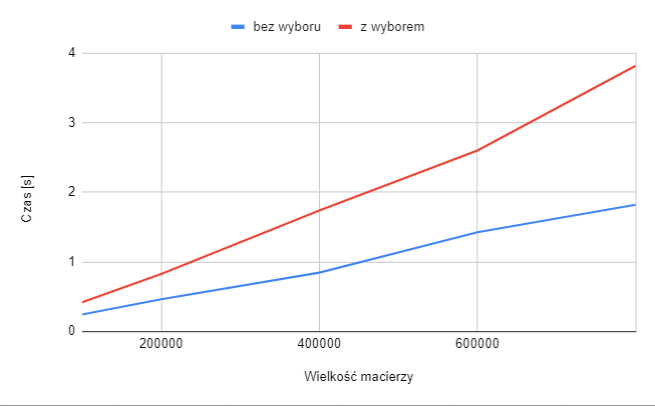
\includegraphics[width=0.9\textwidth]{time.png}}
\end{figure}	
	
\begin{figure}[!htbp]
	\centering
	{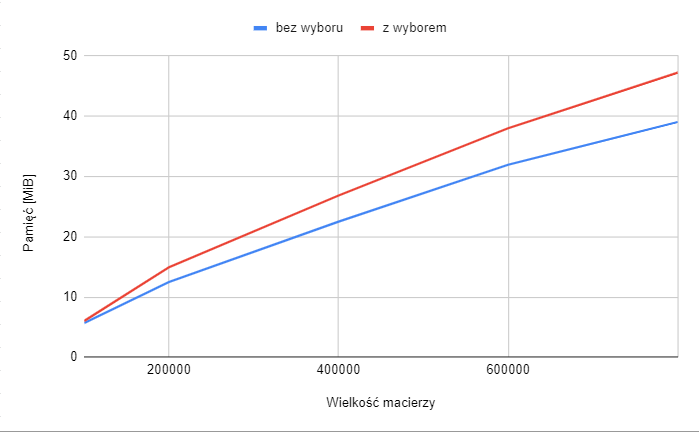
\includegraphics[width=0.9\textwidth]{memory.png}}
\end{figure}	

\subsection{Wnioski}
Wyniki sugerują, że złożoność obliczeniowa zaimplementowanych metod jest liniowa. Co istotne, metoda z wyborem elementu głównego jest wolniejsza i zużywa więcej pamięci niż metoda bez jego wyboru, jednakże daje dokładniejsze wyniki. Warto również wspomnieć, że w przypadku elementów zerowych na diagonali użycie metody z wyborem elementu głównego może być konieczne do rozwiązania układu.

\end{document}